\documentclass[10pt,aspectratio=169]{beamer}
\usetheme{metropolis}
\usepackage{appendixnumberbeamer}
\usepackage{booktabs}
\usepackage{colortbl}
\usepackage{tikz}
\usepackage{amsmath}
\usepackage{xcolor}
\usepackage{graphicx}

\definecolor{good}{RGB}{21,128,61}
\definecolor{bad}{RGB}{185,28,28}
\definecolor{acc}{RGB}{43,108,176}
\definecolor{warn}{RGB}{192,86,33}

\metroset{block=fill,progressbar=frametitle}
\setbeamertemplate{frame numbering}[fraction]

% key-message box
\newcommand{\keybox}[1]{%
  \begin{center}\begin{beamercolorbox}[wd=0.94\textwidth,sep=6pt,rounded=true,shadow=true]{block body}%
  \centering #1
  \end{beamercolorbox}\end{center}}
\newcommand{\gv}[1]{{\color{good}\textbf{#1}}}
\newcommand{\bv}[1]{{\color{bad}\textbf{#1}}}
\newcommand{\ac}[1]{{\color{acc}\textbf{#1}}}

\newcommand{\fig}[2][0.8]{\centering\includegraphics[width=#1\textwidth]{figs/#2}}

\title{P2 BASKET detectors: a lifetime autopsy}
\subtitle{Why det3 and det1 died --- two detectors, two diseases}
\author{Cosmic-bench QA analysis}
\institute{P2 BASKET / Saclay}
\date{19 July 2026}

\begin{document}

\maketitle

\begin{frame}{The question}
Two P2 BASKET Micromegas detectors lost their efficiency to (near) zero during
cosmic-bench running.
\begin{itemize}
  \item \textbf{det3 (P2\_3)} --- died over $\sim$4~h on the evening of 16 July,
        starting from a healthy 76\%.
  \item \textbf{det1 (P2\_1)} --- intermittent since 1 July: dead, then
        \emph{revives} for a couple of hours at night, then dies again.
\end{itemize}
\vfill
\keybox{\large Same detector design, same gas line, same DAQ. \\[2pt]
Are these the \emph{same} failure? \bv{No} --- and the data tell us exactly why.}
\vfill
\footnotesize This talk: the observations, the forensic method, and a
step-by-step diagnosis leading to two distinct, actionable root causes.
\end{frame}

\begin{frame}{The setup in one slide}
\begin{columns}
\begin{column}{0.58\textwidth}
\textbf{The detector (P2 BASKET wedge)}
\begin{itemize}\footnotesize
  \item Metallic (non-resistive) Micromegas, \textbf{pad} readout, fan geometry
        split into connectors 1--10.
  \item \textbf{Amplification} gap $\sim$128\,\textmu m (mesh$\to$anode).
  \item \textbf{Drift} gap 3\,mm; drift electrode = aluminized mylar window.
  \item Gas: \textbf{Ar/iC$_4$H$_{10}$ 95/5} from a mixer; gas \textbf{in} at the
        connector-1 corner, \textbf{out} at connector 10.
\end{itemize}
\textbf{The measurement}
\begin{itemize}\footnotesize
  \item \textbf{M3} scintillator/telescope = external reference track.
  \item Efficiency $=$ fraction of clean M3 tracks with a matched P2 cluster
        ($<$40\,mm), in a frozen active area.
  \item DREAM DAQ $\to$ pad hits \emph{and} full waveforms (60\,ns/sample).
\end{itemize}
\end{column}
\begin{column}{0.42\textwidth}
\centering
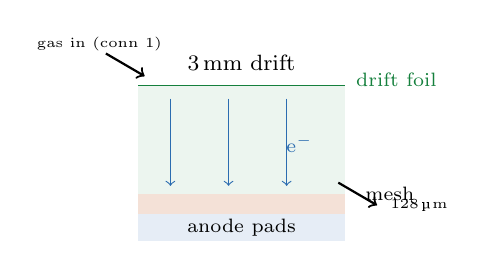
\begin{tikzpicture}[scale=0.82,font=\scriptsize]
  \fill[acc!12] (0,0) rectangle (3.2,0.42); \node at (1.6,0.21){anode pads};
  \draw[thick] (0,0.72) -- (3.2,0.72); \node at (3.9,0.72){mesh};
  \fill[warn!18] (0,0.42) rectangle (3.2,0.72); \node at (4.35,0.55){\tiny 128\,\textmu m};
  \draw[good,thick] (0,2.4) -- (3.2,2.4); \node at (4.0,2.5){\color{good}drift foil};
  \fill[good!8] (0,0.72) rectangle (3.2,2.4);
  \draw[->,acc] (0.5,2.2) -- (0.5,0.85); \draw[->,acc] (1.4,2.2) -- (1.4,0.85);
  \draw[->,acc] (2.3,2.2) -- (2.3,0.85); \node[acc] at (2.5,1.5){e$^-$};
  \node at (1.6,2.75){\footnotesize 3\,mm drift};
  \draw[<-,thick] (0.1,2.55) -- (-0.5,2.9); \node at (-0.6,3.05){\tiny gas in (conn 1)};
  \draw[->,thick] (3.1,0.9) -- (3.7,0.55);
\end{tikzpicture}
\vfill
\footnotesize A muon ionises the 3\,mm gap; electrons drift down, avalanche in
the thin gap, induce a pad signal.
\end{column}
\end{columns}
\end{frame}

\begin{frame}{Before anything: a data-quality trap we had to fix}
\begin{columns}
\begin{column}{0.62\textwidth}
The online hit-builder assigns each file to an FEU by a regex on the filename.
The \textbf{new run names contain the voltages}:
\begin{center}\small\texttt{...det3\_\bv{420\_82}0...} $\Rightarrow$ ``FEU 82''\end{center}
\begin{itemize}\footnotesize
  \item No FEU-82 pedestal exists $\Rightarrow$ fell back to
        ``assume zero-suppressed, RMS $=1$'' $\Rightarrow$ 5 ADC threshold.
  \item Result: an \textbf{18 ADC noise ``wallpaper''} on every pad
        ($\sim$600 hits/event) burying the real signal.
  \item Old run names had a ``V'' (\texttt{mesh\_395V}) $\Rightarrow$ det1/det2
        were never affected.
\end{itemize}
\alert{Fix:} all 29 det3 sub-runs \textbf{reprocessed} with the correct
contemporaneous pedestals (148 file$\leftrightarrow$pedestal pairs, 0 mismatches);
watcher regex patched \& restarted.
\end{column}
\begin{column}{0.38\textwidth}
\keybox{\footnotesize The pedestals \emph{themselves} were fine:\\
12h06 vs 19h40 sets agree to \gv{$\le$0.4 ADC}/channel, RMS 5.6--5.8.\\[4pt]
Every result in this talk uses \gv{clean, re-pedestalled} data,
\texttt{min\_amp}=0.}
\vspace{4pt}
\footnotesize This was a \emph{reconstruction} artefact, not a detector effect
--- but it had to be removed before any autopsy.
\end{column}
\end{columns}
\end{frame}

% ============================================================= PART I
\section{det3: the observation}

\begin{frame}{The det3 lifetime timeline --- the whole story on one axis}
\fig[0.78]{lifetime_master.png}
\end{frame}

\begin{frame}{Reading the timeline --- step by step}
\begin{columns}
\begin{column}{0.5\textwidth}
\textbf{Panel 1 --- efficiency}
\begin{itemize}\footnotesize
  \item \gv{75--77\% plateau, stable 4~h} (drift scan, afternoon).
  \item HV off 17:47--19:42 (run gap).
  \item \ac{Returns at full 76\% at 19:43} --- the HV cycle did \emph{not}
        break it.
  \item \bv{Monotonic decay from $\sim$20:00}, $\tau\approx2$~h, to $\sim$1\%.
  \item 10~h next day at the same HV: \bv{dead, no recovery}.
\end{itemize}
\end{column}
\begin{column}{0.5\textwidth}
\textbf{Panels 2--4 --- context}
\begin{itemize}\footnotesize
  \item Panel 2: matched cluster charge \emph{collapses} with the efficiency.
  \item Panel 3: \gv{M3 reference is flat} --- 5.5--5.9 Hz, 42--45\%
        good tracks. The DAQ/reference is innocent.
  \item Panel 4: det4 (shared gas) --- control.
\end{itemize}
\end{column}
\end{columns}
\vfill
\keybox{The death is \bv{real}, \bv{gradual}, and \bv{not triggered by HV};
the reference proves it is det3 itself that changed.}
\end{frame}

% ============================================================= PART II
\section{det3: the forensic toolkit}

\begin{frame}{Tool 1 --- gain: the avalanche is collapsing}
\begin{columns}
\begin{column}{0.55\textwidth}
\fig[1.0]{amp_spectra_periods.png}
\end{column}
\begin{column}{0.45\textwidth}
Matched-cluster charge, per period:
\begin{itemize}\footnotesize
  \item healthy afternoon: \gv{med 610 ADC}
  \item initial run (19:43): 412
  \item 21:45: 247
  \item final run: \bv{128} (threshold-limited remnant --- true loss even larger)
\end{itemize}
\vspace{4pt}
The whole Landau slides left: this is a \textbf{gain} loss, not a dead-channel
or mapping problem.
\end{column}
\end{columns}
\end{frame}

\begin{frame}{Tool 2 --- space: the death is NOT uniform}
\fig[0.98]{spatial_periods.png}
\vspace{-2pt}
\footnotesize At 21:45 the connector-2 edge is at 20--40\% while connectors 6--7
still hold 60--80\%. \bv{A front sweeps across the plane over hours.}
\end{frame}

\begin{frame}{Tool 2 --- the front, in detector coordinates}
\fig[0.86]{front_timelapse_detframe.png}
\end{frame}

\begin{frame}{Tool 2 --- the front moves \emph{with the gas flow}}
\begin{columns}
\begin{column}{0.56\textwidth}
\fig[1.0]{front_connector_lag.png}
\end{column}
\begin{column}{0.44\textwidth}
Time each connector drops below 60\% of its healthy amplitude:
\begin{itemize}\footnotesize
  \item conn 2 (next to inlet): \bv{20:55}
  \item conn 3--4: 21:05
  \item conn 5--6--7 (toward outlet): 21:15
\end{itemize}
\vspace{4pt}
A coherent \textbf{$\sim$40-minute traversal} of the wedge, inlet $\to$ outlet.
\keybox{\footnotesize Nothing electrical crawls across a plane at mm/minute.
\gv{A moving gas front does.}}
\end{column}
\end{columns}
\end{frame}

\begin{frame}{Tool 3 --- time: the drift is slowing down}
\begin{columns}
\begin{column}{0.5\textwidth}
\fig[1.0]{drift_time_shift.png}
\end{column}
\begin{column}{0.5\textwidth}
At \textbf{fixed pulse amplitude} (150--500 ADC, so gain-independent), the
waveform peak arrival moves:
\begin{itemize}\footnotesize
  \item early initial run: sample 12.0
  \item late initial run: sample 16.4
  \item $\Rightarrow$ \bv{+260 ns later}, rise time 240$\to$300 ns.
\end{itemize}
\vspace{3pt}
A pure \emph{gas transport} signature: at constant vmon, no HV/mechanical fault
changes the drift time at fixed amplitude.
\end{column}
\end{columns}
\end{frame}

% ============================================================= PART III
\section{det3: two hypotheses, one test}

\begin{frame}{Two candidate mechanisms}
\begin{columns}
\begin{column}{0.5\textwidth}
\textbf{(A) Drift-foil HV decoupling}
\begin{itemize}\footnotesize
  \item Aluminized-mylar drift electrode loses contact with its HV feed.
  \item Drift field collapses; no current flows $\Rightarrow$ \emph{invisible to
        vmon}.
  \item Would explain gain loss + late arrivals via a falling drift field.
\end{itemize}
\end{column}
\begin{column}{0.5\textwidth}
\textbf{(B) Gas contamination}
\begin{itemize}\footnotesize
  \item Bad gas (water/air/wrong mix) enters at the inlet and displaces the good
        fill.
  \item Changes drift velocity \emph{and} avalanche behaviour.
  \item Naturally produces a moving front tied to flow.
\end{itemize}
\end{column}
\end{columns}
\vfill
\keybox{Both fit the timeline. We need a test that \emph{separates} them ---
and a warning about a test that does \bv{not}.}
\end{frame}

\begin{frame}{The tempting-but-degenerate test}
\begin{columns}
\begin{column}{0.52\textwidth}
\fig[1.0]{drift_ladder_trajectory.png}
\end{column}
\begin{column}{0.48\textwidth}
The dying detector \emph{retraces} the healthy drift-voltage ladder in
\textbf{all three} observables at once (arrival time, charge, efficiency).
\vspace{4pt}
Tempting conclusion: ``the drift field is collapsing.''
\vspace{6pt}
\alert{But this is degenerate.} All three observables are driven by one latent
variable --- the \textbf{charge-arrival duration vs the shaper} (ballistic
deficit). The ladder moves it via $E$; contamination moves it via $v(E)$. \\[3pt]
\bv{Landing on the ladder proves nothing about which knob moved.}
\end{column}
\end{columns}
\end{frame}

\begin{frame}{What breaks the tie: the contact geometry}
\begin{columns}
\begin{column}{0.58\textwidth}
The drift-HV contact is at the \textbf{connector-1 corner} (outer radius) ---
right next to \textbf{connector 2, which died \emph{first}}.
\vspace{6pt}
Every electrical-decoupling topology predicts the \bv{opposite}:
\begin{itemize}\footnotesize
  \item intact aluminised sheet $=$ equipotential $\Rightarrow$ uniform death;
  \item fragmenting metallisation $\Rightarrow$ the \emph{far} patches die first.
\end{itemize}
There is no wiring of that foil that kills the near-contact region first.
\end{column}
\begin{column}{0.42\textwidth}
\keybox{\footnotesize Front direction $=$ gas flow (inlet conn 1 $\to$ outlet
conn 10), \emph{not} distance from the HV contact.\\[4pt]
$\Rightarrow$ Hypothesis (A) \bv{falsified}.}
\vspace{4pt}
\footnotesize (The inlet-corner start likely marks where inflation stress is
largest, i.e. where fresh gas first enters --- not a foil defect.)
\end{column}
\end{columns}
\end{frame}

% ============================================================= PART IV
\section{det3: naming the gas}

\begin{frame}{Magboltz --- can any contaminant do this?}
\fig[0.96]{magboltz_composition_comparison.png}
\vspace{-2pt}
\footnotesize Left: at our drift field \emph{every} contaminant makes the drift
\emph{faster} (nominal 95/5 is the slowest). A naive ``dry-gas'' contamination
cannot explain \emph{late} arrivals --- we need the low-field behaviour.
\end{frame}

\begin{frame}{Magboltz $v(E)$ --- the ladder fingerprints WATER}
\begin{columns}
\begin{column}{0.62\textwidth}
\fig[1.0]{magboltz_vE_curves_vs_ladder.png}
\end{column}
\begin{column}{0.38\textwidth}
\textbf{Middle panel is the match:}
\begin{itemize}\footnotesize
  \item measured ladder: \bv{+446 ns} at $\Delta V{=}50$, +133 at 100.
  \item every \emph{dry} mix: $\le$+40 ns.
  \item \gv{H$_2$O $\approx$ 2\%}: +359 / +93 ns --- right shape, right size.
\end{itemize}
Only water-class mixtures have the strongly \emph{rising} low-field $v(E)$ the
ladder demands.
\vspace{3pt}
Right panel: if it is humid \emph{air}, O$_2$ attachment eats 20--100\% of the
charge --- a second killer.
\end{column}
\end{columns}
\end{frame}

\begin{frame}{det3 verdict}
\keybox{\Large \bv{Gas: a water-class contamination front.}}
\vspace{2pt}
\begin{itemize}\footnotesize
  \item \gv{Chronic:} percent-level water was present already in the ``healthy''
        afternoon (the ladder timing is not clean 95/5; matches the July
        ``drift 2$\times$ slow'' finding).
  \item \bv{Acute:} contamination rose sharply $\sim$20:00 on 16 July; a front
        entered at the inlet, swept the wedge in $\sim$40--60 min/pass, detector
        fully contaminated by midnight, no recovery while the same gas flowed.
  \item Why the amplitude collapses without a Townsend collapse:
        \textbf{ballistic deficit} --- slow charge arrival ($\gg$ shaping time)
        suppresses the measured peak at constant avalanche gain.
\end{itemize}
\vfill
\footnotesize Consistent with: no sparks, quiet mesh current, gradual $\tau\sim$2\,h
decay, front tied to flow, and the drift-time increase.
\end{frame}

% ============================================================= PART V
\section{det1: does the same story hold?}

\begin{frame}{det1 is a different animal --- the intermittency}
\begin{columns}
\begin{column}{0.5\textwidth}
det1 has been \textbf{intermittent} since 1 July:
\begin{itemize}\footnotesize
  \item baseline dead ($\sim$4\%),
  \item \gv{revives to 50--63\% for $\sim$2 h at night},
  \item then dies again.
\end{itemize}
A gas front cannot switch a detector back \emph{on}. So we apply the same
toolkit and ask: same disease, or different?
\end{column}
\begin{column}{0.5\textwidth}
\fig[1.0]{det1_revival_per_connector.png}
\end{column}
\end{columns}
\vspace{2pt}
\footnotesize The 7-8 night revival switches on \bv{globally} --- all 8
connectors cross 50\% within one 10-min bin. That is an \emph{electrical
reconnection}, not a diffusing gas.
\end{frame}

\begin{frame}{The discriminator: arrival time, dead vs alive}
\begin{columns}
\begin{column}{0.56\textwidth}
\fig[1.0]{det1_vs_det3_timing_discriminator.png}
\end{column}
\begin{column}{0.44\textwidth}
Same fixed-amplitude waveform test, opposite result:
\begin{itemize}\footnotesize
  \item \textbf{det3} dead phases arrive \bv{LATE} ($+$7--9 samples)
        $\Rightarrow$ slow drift $\Rightarrow$ gas.
  \item \textbf{det1} dead phases arrive \gv{EARLY} ($-$2 samples: 6.0 vs
        alive 8.0).
\end{itemize}
\vspace{4pt}
Early arrivals $\Rightarrow$ drift field \emph{up}. If the \textbf{mesh
potential sags} (bad contact, mesh drifts toward the anode): amplification
$\downarrow$ (dead) \emph{and} drift-to-mesh $\Delta V\uparrow$
$\Rightarrow$ faster drift.
\end{column}
\end{columns}
\end{frame}

\begin{frame}{det1 --- the HV current confirms it}
\begin{columns}
\begin{column}{0.5\textwidth}
\textbf{At the moment of death (1 July):}
\begin{itemize}\footnotesize
  \item vmon steady (mesh 420, drift 600).
  \item mesh \bv{imon spikes 1--3 $\to$ 8\,\textmu A} exactly at death, and
        stays spiky afterwards.
  \item Current spikes \emph{with low chamber gain} $=$ \textbf{arcing at the
        failing contact}, not chamber discharges.
\end{itemize}
\vspace{4pt}
$\Rightarrow$ det1's ``sparks'' in the dead state were the \textbf{contact},
not the gas.
\end{column}
\begin{column}{0.5\textwidth}
\fig[1.0]{det1_death_per_connector.png}\\
\footnotesize The original death is also \bv{simultaneous} across all 9
connectors ($t_{50}$ spread $<$15 min) --- a global electrical mechanism, no
front.
\end{column}
\end{columns}
\end{frame}

\begin{frame}{det1 verdict}
\keybox{\Large \bv{Electrical: a failing mesh-HV contact.}}
\vspace{4pt}
\begin{itemize}\footnotesize
  \item Early dead-phase arrivals $\Rightarrow$ mesh potential sagging (drift
        field up while gain down).
  \item Global, instantaneous on/off (revival + death) $\Rightarrow$ a contact
        reconnecting/breaking (plausibly thermal --- night revivals).
  \item imon arcing at the death moment $\Rightarrow$ current across the failing
        joint.
\end{itemize}
\vfill
\footnotesize This \emph{confirms} the leading hypothesis of the July
intermittency report --- now with a waveform-level discriminator that did not
exist then.
\end{frame}

% ============================================================= PART VI
\section{Putting it together}

\begin{frame}{Two detectors, two diseases --- side by side}
\centering\small
\begin{tabular}{lll}
\toprule
signature & \textbf{det3} (16 Jul) & \textbf{det1} (1 Jul / 8 Jul) \\
\midrule
stable before death & 75--77\%, 4\,h & 70--73\%, 8.5\,h \\
collapse $\tau$ & $\sim$2\,h & $\sim$1.5\,h \\
\rowcolor{black!6} arrival, dead phase & \bv{LATE} ($+$260\,ns) & \gv{EARLY} ($-$120\,ns) \\
spatial pattern & ordered front (40\,min) & simultaneous ($<$15\,min) \\
\rowcolor{black!6} mesh current at death & silent, no sparks & spikes to 8\,\textmu A \\
recovery & never & intermittent revivals \\
\midrule
\textbf{verdict} & \bv{gas: water contamination} & \bv{electrical: mesh contact} \\
\bottomrule
\end{tabular}
\vfill
\keybox{The timeline made these separable: \gv{det2 ran at 65\% on the same gas
9--12 July} --- the bench gas was fine a week \emph{after} det1 died, and went
bad only around 16 July. \textbf{Two failures, two causes, two dates, no
contradiction.}}
\end{frame}

\begin{frame}{The full timeline}
\centering
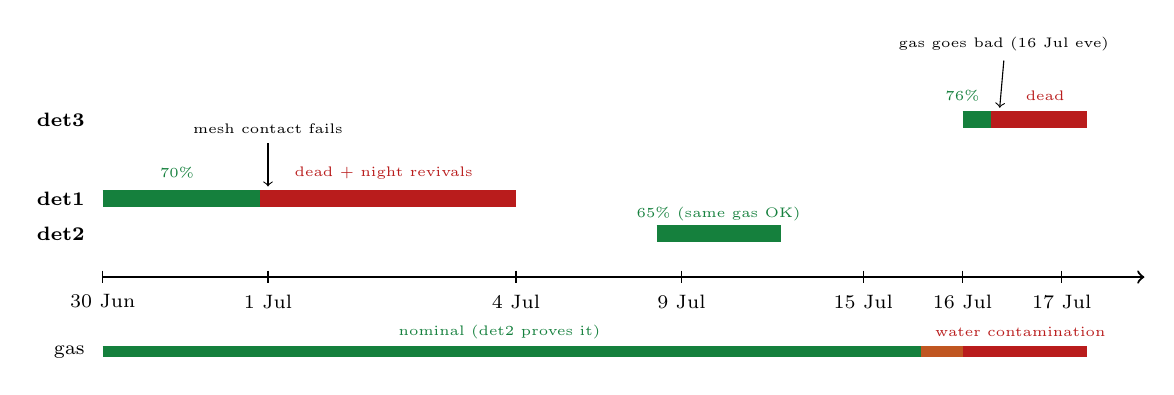
\begin{tikzpicture}[font=\scriptsize,x=1.05cm]
% axis
\draw[->,thick] (0,0) -- (12.6,0);
\foreach \x/\l in {0/{30 Jun},2/{1 Jul},5/{4 Jul},7/{9 Jul},9.2/{15 Jul},10.4/{16 Jul},11.6/{17 Jul}}
  {\draw (\x,0.08) -- (\x,-0.08); \node[below] at (\x,-0.1){\l};}
% det1 band
\node[left] at (-0.1,1.0){\textbf{det1}};
\draw[good,line width=6pt] (0,1.0) -- (1.9,1.0);
\draw[bad,line width=6pt] (1.9,1.0) -- (5.0,1.0);
\node[good] at (0.9,1.32){\tiny 70\%};
\node[bad] at (3.4,1.32){\tiny dead + night revivals};
\draw[->] (2.0,1.7) -- (2.0,1.15); \node[above] at (2.0,1.7){\tiny mesh contact fails};
% det2 band
\node[left] at (-0.1,0.55){\textbf{det2}};
\draw[good,line width=6pt] (6.7,0.55) -- (8.2,0.55);
\node[good] at (7.45,0.8){\tiny 65\% (same gas OK)};
% det3 band
\node[left] at (-0.1,2.0){\textbf{det3}};
\draw[good,line width=6pt] (10.4,2.0) -- (10.75,2.0);
\draw[bad,line width=6pt] (10.75,2.0) -- (11.9,2.0);
\node[good] at (10.4,2.3){\tiny 76\%};
\node[bad] at (11.4,2.3){\tiny dead};
\draw[->] (10.9,2.75) -- (10.85,2.15); \node[above] at (10.9,2.75){\tiny gas goes bad (16 Jul eve)};
% gas health strip
\node[left] at (-0.1,-0.95){\scriptsize gas};
\draw[good,line width=4pt] (0,-0.95) -- (9.9,-0.95);
\draw[warn,line width=4pt] (9.9,-0.95) -- (10.4,-0.95);
\draw[bad,line width=4pt] (10.4,-0.95) -- (11.9,-0.95);
\node[good] at (4.8,-0.7){\tiny nominal (det2 proves it)};
\node[bad] at (11.1,-0.7){\tiny water contamination};
\end{tikzpicture}
\vfill
\footnotesize The gas was healthy through det1's death and det2's run; it
degraded only in mid-July, which is what killed det3. det1's failure is
independent and electrical.
\end{frame}

\begin{frame}{Actions \& lessons}
\begin{columns}
\begin{column}{0.5\textwidth}
\textbf{det3 (gas)}
\begin{enumerate}\footnotesize
  \item \ac{Dew-point / moisture meter} on the det3 line --- minutes, decisive.
  \item Inspect bubbler, iC$_4$H$_{10}$ bottle, fittings opened $\sim$16 Jul.
  \item \gv{Flush with dry premix} + 30-min run: if it revives, gas confirmed,
        detector undamaged.
  \item Log mixer MFC flows with the HV stream.
\end{enumerate}
\end{column}
\begin{column}{0.5\textwidth}
\textbf{det1 (electrical)}
\begin{enumerate}\footnotesize
  \item \ac{Rework the mesh-HV contact.}
  \item \gv{Induced-pulse test} on the mesh line before/after
        (step HV, look for the induced spike) to verify.
\end{enumerate}
\vspace{6pt}
\textbf{For the series}
\begin{itemize}\footnotesize
  \item Both faults live at the \bv{HV/gas interfaces} of the foil/mesh
        assembly.
  \item Design review of the contact scheme + drift-window sandwich before
        det5+.
\end{itemize}
\end{column}
\end{columns}
\end{frame}

\begin{frame}[standout]
Two detectors, two diseases.\\[6pt]
{\large det3 $=$ \textbf{gas (water)} \quad\textbullet\quad det1 $=$ \textbf{mesh contact}}\\[10pt]
{\normalsize The waveform arrival time --- late vs early --- was the key that
separated them.}
\end{frame}

\appendix
\begin{frame}{Backup --- effective drift voltage vs time (det3)}
\fig[0.72]{veff_timeline.png}\\
\footnotesize The gain-implied ``effective mesh voltage'' from the mesh-scan
calibration --- a lower bound; illustrates the smooth collapse.
\end{frame}

\begin{frame}{Backup --- method notes}
\footnotesize
\begin{itemize}
  \item All efficiencies: one \emph{frozen} pad$\to$M3 transform (fit on the
        healthy initial run), match radius 40\,mm, active-area 30\,mm, clean
        re-pedestalled data, \texttt{min\_amp}=0.
  \item Waveform timing: pedestal- and common-noise-subtracted decoded
        waveforms; peak sample via arg-max on a fixed 150--500 ADC amplitude
        window to decouple timing from gain.
  \item Magboltz: Garfield++ on lxplus, Ar/iC$_4$H$_{10}$ 95/5 $\pm$ admixtures,
        drift field 1333 V/cm, amplification 32.8 kV/cm.
  \item Data: pipeline stages 02--17; autopsy stage \texttt{17\_lifetime\_autopsy.py};
        reports in \texttt{Analysis/det3/lifetime\_autopsy/} and
        \texttt{Analysis/det1/lifetime\_autopsy/}.
\end{itemize}
\end{frame}

\end{document}
